% =======================================================================================
\section{Network}
\label{app:network}
% =======================================================================================

The network has two outputs (\cref{app:fm}). From the input $y$ and the window centre $\fw$ alone
it returns the frame, a mean and a log standard deviation per coordinate of each source slot; from
a point $Z_t$ in that frame and the flow time $t$ it returns the mean and log standard deviation of
the endpoint $Z_1$. It is a transformer with two sides: the \ac{mmdit} of \citet{esser2024scaling},
with the adaptive-normalisation conditioning of \citet{peebles2023scalable}, made one-way. The
encoder runs the data tokens and one frame register per slot, conditioned on the window alone; its
keys and values in every block, and the frame, depend on the observation only and are computed
once for it. The decoder runs the source tokens and \NetworkSinksWord{} sink tokens, conditioned on
the flow time and the window, attending to each other and to the cached data and registers.
\Acp{rope} put the data and the sources on one frequency axis. \Cref{fig:network-architecture}
shows the network and \cref{tab:network-sizes} its sizes. Transformers also condition posterior
estimators for ground-based detectors \citep{kofler2026flexible}; here the sources are tokens too,
and attend to the data and to each other.

\begin{figure*}[t]
  \centering
  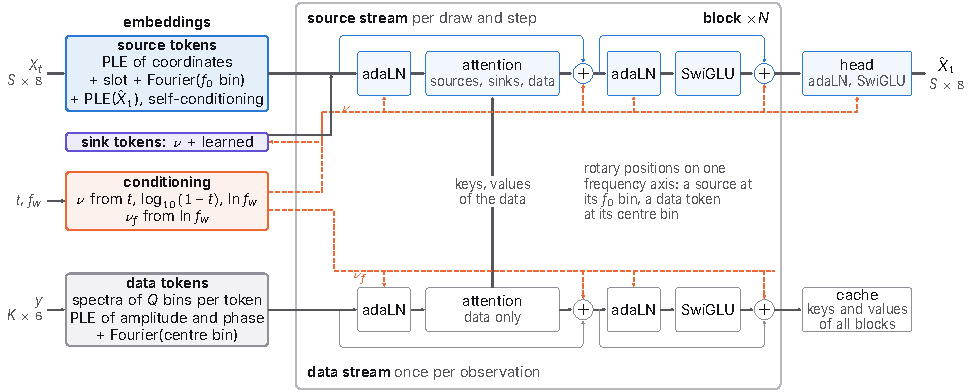
\includegraphics[width=\textwidth]{figures/architecture.pdf}
  \caption{The network. The source stream (blue) has one token per source slot, in order of $f_0$;
  the data stream (grey) has one token per \NetworkPatch{} frequency bins of the window, and runs
  with one frame register per slot, which the frame head reads; the sink tokens (violet) join the
  source stream. Conditioning (orange, dashed) modulates every normalisation and residual gate:
  $\nu$ from the flow time and the window in the source stream and head, $\nu_f$ from the window
  alone in the data stream, the registers and the frame head. The data side never reads the
  sources, so its keys and values and the frame are computed once per observation and serve every
  draw and sampler step. Rotary positions place each source at its $f_0$ and each data token at its
  centre frequency.}
  \label{fig:network-architecture}
\end{figure*}

% ---------------------------------------------------------------------------------------
\subsection{Input}
\label{app:network-input}

The network sees a window through three operations: whitening, an \ac{stft} into tokens, and a
compression of the dynamic range.

\paragraph{Whitening.}
The input $y$ is the window whitened by \cref{eq:noise-whiten}: the real and imaginary parts of
$A$, $E$ and $T$ in each of the $K$ bins, $K\times6$ numbers, from the window start $k_0$
(\cref{app:forward-model}). Below, $y_{k,c}$ is the complex whitened value of bin $k =
0,\dots,K-1$ and channel $c\in\{A, E, T\}$. Under noise alone its real and imaginary parts have
unit variance, and a source's whitened signal $\hat h$ has $\sum_{k,c}|\hat h_{k,c}|^2 =
\snr^2$ (\cref{eq:inner}).

\paragraph{Short-time spectra.}
The window is cut into bands of $Q=\NetworkPatch{}$ consecutive bins, one token each:
\NetworkTokensNarrow{} tokens on the narrow band ($K=\NetworkBinsNarrow{}$) and
\NetworkTokensFull{} on the full band ($K=\NetworkBinsFull{}$). An orthonormal inverse discrete
Fourier transform over each band turns its spectrum into $Q$ time samples of the band's signal,
per channel,
\begin{equation}
  \check y_{n,j,c} = \frac{1}{\sqrt Q}\sum_{l=0}^{Q-1} y_{nQ+l,\,c}\,e^{2\pi\ii jl/Q},
  \qquad j = 0,\dots,Q-1,
  \label{eq:network-stft}
\end{equation}
an \ac{stft} with the tokens as its bands. It is critically sampled and untapered, so it is
invertible, keeps the noise white, and neither leaks nor duplicates power between tokens, as an
overlapping tapered transform would. Within a token, a source's sub-bin frequency becomes a
phase slope over the samples, its initial phase the intercept, and the annual Doppler and
amplitude modulation that carry the sky a slow evolution in time.

\paragraph{Compression.}
The transform is unitary, so a source's samples carry the same $\snr^2$ as its bins and a single
sample of its signal has $|\check h| \le \snr$, which reaches \NetworkSnrTop{} at the prior's \qty{\NetworkSnrQuantile}{\percent}
quantile in the full band (\cref{app:priors}), against unit-variance noise. Each complex sample enters as its compressed
amplitude $\operatorname{asinh}|\check y|$, linear in the noise and logarithmic for loud signals,
and its gated phase $\check y/\sqrt{1+|\check y|^2}$, which is $\check y$ in the noise and a unit
phasor for a loud signal. A token is thus $3Q\times3 = \NetworkTokenScalars{}$ numbers:
\NetworkAmplitudeScalars{} amplitudes and \NetworkPhaseScalars{} phase parts.

\paragraph{Absolute frequency.}
Whitening and windowing remove the absolute frequency, which still matters: the Doppler width
scales with $f$ and the prior's typical drift $\fdot$ with $f_0^{\ChartFdotSlope}$ (\cref{app:chart}). Each data token is therefore given the
absolute frequencies of its lowest and highest bin, $(k_0 + nQ)/\Tobs$ and $(k_0 + nQ + Q - 1)/\Tobs$,
and the whole network the window's range of $f_0$ (\cref{app:network-embeddings}).

% ---------------------------------------------------------------------------------------
\subsection{Embeddings}
\label{app:network-embeddings}

All feed-forward maps are SwiGLU \citep{shazeer2020glu}, $\mathrm{FF}(h) =
W_2\bigl(a\odot\mathrm{SiLU}(g)\bigr)$ with $[a;g] = W_1h$. Scalars enter in one of two ways
(\cref{tab:network-embeddings}). The \NetworkTokenScalars{} numbers of a data token, already
compressed, and the \NetworkSourceScalars{} numbers of a source token, already in the frame, are
mapped linearly to $\R^D$. A frequency or a time enters as sinusoids, $E(\xi) =
\bigl[\cos(2\pi\xi/P_k);\ \sin(2\pi\xi/P_k)\bigr]_k$ over a set of periods $P_k$, followed by an
$\mathrm{FF}$. The absolute frequencies of the data tokens, the sources and the window share one
set of periods in hertz, octaves $P_k = 2^kP_0$ from $P_0 = \NetworkFreqFinest{}$ of a bin
($1/\Tobs$) up to past twice the top bin of the band; their turns $\xi/P_k$ are reduced modulo one
in float64 before the cast, so even the finest period keeps its phase. Every embedding runs in
float32, whatever the backbone's precision (\cref{app:network-sizes}).

\begin{table*}[t]
  \centering
  \caption{What each token is built from. Sinusoidal embeddings of a frequency use periods
  octave-spaced in hertz from \NetworkFreqFinest{} of a bin up to past twice the top bin of the
  band (counts for the narrow and full band).}
  \label{tab:network-embeddings}
  \small
  \begin{tabular}{@{}lll@{}}
    \toprule
    input & embedding & numbers or periods \\
    \midrule
    \multicolumn{3}{@{}l}{\emph{data token}} \\
    amplitudes and phase parts & linear & \NetworkTokenScalars{} numbers \\
    lowest and highest frequency & sinusoidal, $\mathrm{FF}_y$ & \NetworkFreqPeriodsNarrow{} / \NetworkFreqPeriodsFull{} periods each \\
    \midrule
    \multicolumn{3}{@{}l}{\emph{frame register}} \\
    slot & learned & one vector per slot, plus $\nu_f$ \\
    \midrule
    \multicolumn{3}{@{}l}{\emph{source token}} \\
    $Z$, $X$, harmonics, $\mu$, $\log\sigma$ & linear & \NetworkSourceScalars{} numbers \\
    $f_0$ & sinusoidal, $\mathrm{FF}_{f_0}$ & \NetworkFreqPeriodsNarrow{} / \NetworkFreqPeriodsFull{} periods \\
    \midrule
    \multicolumn{3}{@{}l}{\emph{conditioning}} \\
    $t$, $\log_{10}(1-t)$ & sinusoidal, $\mathrm{FF}_\nu$ & \NetworkSinusoidFreqs{} over \NetworkSinusoidDecades{} decades each \\
    lowest and highest $f_0$ of the window & sinusoidal, $\mathrm{FF}_f$ & \NetworkFreqPeriodsNarrow{} / \NetworkFreqPeriodsFull{} periods each \\
    \bottomrule
  \end{tabular}
\end{table*}

\paragraph{Sources.}
Each source enters as \NetworkSourceScalars{} scalars: its \NetworkCoordsWord{} coordinates in the
frame, $Z$, and in the chart, $X = \mu + \sigma Z$ (\cref{app:chart}); the higher harmonics of its
two helicity amplitudes in $X$, $r\cos k\phi$ and $r\sin k\phi$ for $k=2,\dots,\NetworkHarmonics{}$,
with $(r,\phi)$ the polar form of each helicity pair (\NetworkHarmonicScalars{} scalars); and its
slot's frame, $\mu$ and $\log\sigma$. The frame enters through a stop-gradient, so the flow cannot
train it (\cref{app:fm-frame}). The harmonics give the network functions of the phases that vanish
with the amplitude. The token adds a sinusoidal embedding of its absolute frequency $f_0$, which
comes from $x_f$ through the inverse chart in float64, before any cast; it carries no learned label
of its slot (\cref{app:network-frame}).

\paragraph{Conditioning.}
The data stream, the registers and the frame head are conditioned on the window alone,
\begin{equation}
  \nu_f = \mathrm{FF}_f\bigl(\bigl[E(f_{\rm lo});\ E(f_{\rm hi})\bigr]\bigr),
\end{equation}
with $f_{\rm lo}$ and $f_{\rm hi}$ in hertz the lowest and highest $f_0$ a source of the window can
have, the prior's range cut to the window less its guard bands (\cref{app:forward-model}). The source stream,
the sinks and the source head are conditioned on
\begin{equation}
  \nu = \mathrm{FF}_\nu\Bigl(\bigl[E(t);\ E\bigl(\max(\log_{10}(1-t), -\NetworkTimeDecades{}) +
  \NetworkTimeDecades{}\bigr)\bigr]\Bigr) + \nu_f,
  \label{eq:network-c}
\end{equation}
where each time scalar's periods are geometric down from twice its span, and $t$ is the path
position $s$ of \cref{app:fm}. The second input resolves the last decades of the path, where the
fine structure of a posterior forms (\cref{app:fm-sensitivity}).

% ---------------------------------------------------------------------------------------
\subsection{One-Way Blocks}
\label{app:network-blocks}

Each of the $N$ blocks updates four streams: the data tokens $h^y$ and the frame registers $h^r$,
conditioned on $\nu_f$, and the source tokens $h^x$ and the sink tokens $h^s$, conditioned on
$\nu$. For each stream $\ell$, a zero-initialised linear map of $\mathrm{SiLU}(\nu_f)$ or
$\mathrm{SiLU}(\nu)$ produces a shift, a scale and a gate, $(\beta^\ell,\gamma^\ell,\varpi^\ell)$,
so that every residual branch starts as the identity and a fresh network ignores its conditioning
\citep{peebles2023scalable}:
\begin{align}
  u^\ell &= \mathrm{LN}(h^\ell)\odot(1+\gamma^\ell) + \beta^\ell,\qquad
  [q^\ell; k^\ell; v^\ell] = \bigl[W^\ell_{q}u^\ell; W^\ell_{k}u^\ell; W^\ell_{v}u^\ell\bigr], \nonumber\\
  [o^y; o^r] &= \mathrm{Attn}\bigl([q^y; q^r];\ [k^y; k^r], [v^y; v^r]\bigr),\nonumber\\
  [o^x; o^s] &= \mathrm{Attn}\bigl([q^x; q^s];\ [k^x; k^s; k^y; k^r], [v^x; v^s; v^y; v^r]\bigr), \nonumber\\
  h^\ell &\leftarrow h^\ell + \varpi^\ell\odot W^\ell_{o}\,o^\ell, \nonumber\\
  h^\ell &\leftarrow h^\ell + \varpi'^\ell\odot\mathrm{FF}^\ell\bigl(\mathrm{LN}(h^\ell)\odot(1+\gamma'^\ell) + \beta'^\ell\bigr),
  \label{eq:network-block}
\end{align}
with a second shift, scale and gate $(\beta'^\ell,\gamma'^\ell,\varpi'^\ell)$ for the
feed-forward branch, $\mathrm{LN}$ a layer normalisation without learned affine parameters, and
feed-forward hidden width $\NetworkExpand{}D$. Each stream has its own maps, and there are no
biases inside the blocks. The query, key and value maps are separate matrices, so the optimiser
orthogonalises each on its own (\cref{app:training}). Activations are rematerialised in the
backward pass \citep{chen2016training}.

\paragraph{The cache.}
The data and the registers never read the sources, the sinks or $t$, so their keys and values in
every block, $(k^y, v^y)$ and $(k^r, v^r)$, and the registers' outputs depend on $(y,\fw)$ alone.
One encoding of an observation gives its frame and serves all \NetworkDraws{} base draws that share
it in training, and in sampling all \NetworkSampleEvals{} evaluations along every draw's path
(\cref{app:fm-sampling}). In B, encoding a full-band window takes \NetworkEncodeGflopFull{} GFLOP
of matrix products, \NetworkEncodeOverDecodeFull{} times one evaluation on the cache
(\NetworkDecodeGflopFull{} GFLOP), and the cache holds \qty{\NetworkCacheMibFull}{\mebi\byte} in
bfloat16; a narrow window takes \NetworkEncodeGflopNarrow{} and \NetworkDecodeGflopNarrow{} GFLOP,
with \qty{\NetworkCacheMibNarrow}{\mebi\byte} of cache. The last block's data and sink outputs
reach nothing, so it has no output projections, feed-forward modulations or feed-forward maps for
them; its register outputs feed the frame head.

\paragraph{Attention.}
Attention has $H$ heads of dimension \NetworkHeadDim{}. Queries and keys are RMS-normalised per
head, and the queries carry a learned per-head gain, initialised to one
\citep{henry2020query,dehghani2023scaling}. The source and sink queries take one softmax over
their own keys and the cached keys, taken in parts that are never concatenated in memory, which
would copy the shared cache once per draw.

\paragraph{Positions.}
The keys, queries and values of the data and source tokens are rotated
\citep{su2024roformer,miyato2024gta}: each of the \NetworkRopePairs{} pairs of a head's dimensions
turns by $2\pi f/P_j$, with periods $P_j = 2K^{j/(\NetworkRopePairs{}-1)}/T$ geometric from 2 bins
to twice the window. A score then depends on how far apart its two tokens are in frequency, and the
weighted sum of rotated values is turned back by the query's own angle, so a value also arrives
relative to its query. A data token's position $f$ is its centre frequency and a source's its
$f_0$, absolute in hertz; the turns $f/P_j$ are reduced modulo one in float64 before the cast. With
positions in frequency a source finds the data tokens near its own $f_0$ by relative distance,
instead of learning where each absolute position sits. The registers and the sinks carry no
position: their keys and values are not rotated, and their outputs are not turned back.

\paragraph{Sinks.}
The \NetworkSinksWord{} sink tokens, each $\nu$ plus a learned embedding, join the source stream
with their own maps. They give the sources' attention somewhere to go other than the data, and
since they start from $\nu$ they can carry per-draw state \citep{xiao2024efficient,darcet2024vision}.
They are neither cached nor read out.

% ---------------------------------------------------------------------------------------
\subsection{Frame Registers}
\label{app:network-frame}

The frame registers are $S$ tokens, one per source slot, each $\nu_f$ plus a learned slot
embedding. They run with the data stream in every block, attend to the data and to each other, and
the data attend to them too; they are registers in the sense of \citet{darcet2024vision}, tokens
that hold global state, here one per source. After the last block a final layer normalisation with
a shift, scale and gate from $\nu_f$, zero-initialised, and a linear map $\R^D\to
\R^{\NetworkHeadOutputs{}}$ without bias give each slot the shift and log scale
$(\delta_\mu,\delta_s)$ of its frame per coordinate (\cref{eq:fm-frame}). The gate starts at zero,
so a fresh network's frame is the prior's moments.

The slots are the sources in order of $f_0$ (\cref{app:chart-slots}): register $k$ learns to frame
the $k$-th lowest source, and source token $k$ reads its frame through $\mu$ and $\log\sigma$ and
its slot's keys and values in the cache. A source token carries no other label of its slot. Every
map applied to a source token is shared across sources, as in set transformers
\citep{zaheer2017deep,lee2019set}, and its rotary position is physical, the bin of its own $f_0$,
so a source attends to the data near its frequency and to the other sources by their distance in
bins.

% ---------------------------------------------------------------------------------------
\subsection{Head}
\label{app:network-head}

The source tokens pass through a final layer normalisation with a shift and scale from $\nu$, and
an $\mathrm{FF}:\R^D\to\R^{\NetworkHeadOutputs{}}$ with hidden width $D$, shared over sources,
which gives each of the \NetworkCoords{} coordinates the mean $\hat Z_1$ and log standard deviation
$\log\tau$ of the endpoint in the frame (\cref{app:fm-loss}). With the frame head of
\cref{app:network-frame}, these are the network's only outputs.

% ---------------------------------------------------------------------------------------
\subsection{Sizes and Precision}
\label{app:network-sizes}

\Cref{tab:network-sizes} gives the five sizes; all have heads of dimension \NetworkHeadDim{}. The
network is the same on both bands apart from the number of data tokens, which adds no parameters,
and the number of periods of the two absolute-frequency embeddings, which makes the narrow-band totals
\numrange{\NetworkNarrowSavedMin}{\NetworkNarrowSavedMax} parameters lower. Each block has $64D^2
+ H$ parameters: each of the four streams, data, frame registers, sources and sinks, has $6D^2$ in
its modulations, $4D^2$ in its attention maps and $6D^2$ in its feed-forward maps, and the queries
carry $H$ gains. The last block lacks $20D^2$ of them, the data and sink streams' output projections
($2D^2$), feed-forward modulations ($6D^2$) and feed-forward maps ($12D^2$), so the backbone has
$N(64D^2 + H) - 20D^2$, which matches the count of the built network.

\begin{table*}[t]
\caption{Network sizes. Backbone parameters are $N(64D^2 + H) - 20D^2$; the embeddings, the
conditioning maps and the two heads add the rest. The source stream has \NetworkSourcesWord{}
source and \NetworkSinksWord{} sink tokens and the encoder \NetworkSourcesWord{} frame registers
on both bands; the data stream has
\NetworkTokensNarrow{} tokens on the narrow band and \NetworkTokensFull{} on the full band.}
\label{tab:network-sizes}
\centering
\small
\begin{tabular}{@{}lrrrrrr@{}}
\toprule
size & width $D$ & heads $H$ & blocks $N$ & backbone & total (narrow) & total (full) \\
\midrule
XS & \NetworkXsWidth{} & \NetworkXsHeads{} & \NetworkXsBlocks{} & \num{\NetworkXsBackbone} & \num{\NetworkXsTotalNarrow} & \num{\NetworkXsTotalFull} \\
S  & \NetworkSWidth{}  & \NetworkSHeads{}  & \NetworkSBlocks{}  & \num{\NetworkSBackbone}  & \num{\NetworkSTotalNarrow}  & \num{\NetworkSTotalFull} \\
B  & \NetworkBWidth{}  & \NetworkBHeads{}  & \NetworkBBlocks{}  & \num{\NetworkBBackbone}  & \num{\NetworkBTotalNarrow}  & \num{\NetworkBTotalFull} \\
L  & \NetworkLWidth{}  & \NetworkLHeads{}  & \NetworkLBlocks{}  & \num{\NetworkLBackbone}  & \num{\NetworkLTotalNarrow}  & \num{\NetworkLTotalFull} \\
XL & \NetworkXlWidth{} & \NetworkXlHeads{} & \NetworkXlBlocks{} & \num{\NetworkXlBackbone} & \num{\NetworkXlTotalNarrow} & \num{\NetworkXlTotalFull} \\
\bottomrule
\end{tabular}
\end{table*}

\paragraph{Precision.}
Parameters are kept in float32. One setting chooses what runs in bfloat16
\citep{micikevicius2018mixed,kalamkar2019study}: the whole backbone, forward and backward (the
default), only the attention scores and weighted sums, or nothing. In every mode the embeddings,
the conditioning maps and the two heads run in float32, and every softmax is taken in float32. The
embeddings stay in float32 because bfloat16 keeps \NetworkBfBits{} significant bits: rounding a
whitened value above \NetworkBfUnity{} can move it by a unit of noise, and the loudest
samples reach \NetworkSnrTop{}. The source stream's attention logits are computed in float32 from
bfloat16 inputs; it has only \NetworkSourcesWord{} source and \NetworkSinksWord{} sink queries
per draw. In bfloat16 on Ampere or newer GPUs the data stream's self-attention runs as a fused
flash-attention kernel \citep{dao2022flashattention}, so its logits are never materialised.
\textcolor{red}{TODO(new runs): narrow-B/full-B scorecard with a float32 backbone at evaluation.}
